\chapter{Especificación de requisitos}\label{cap:especificación}

El primer paso para el desarrollo de un sistema es la definición de los requisitos que este debe cumplir. Estos son las características y funcionalidades que el sistema debe tener para satisfacer las necesidades de los usuarios finales y cumplir con los objetivos del proyecto. \newline
Para definir estos, se han utilizado diferentes técnicas de recopilación de información, como entrevistas, encuestas y análisis de documentos existentes. 

\Juanlu[]{Si sacas una espada, asegurate de que la enfundas llena de sangre.}

\Juanlu[]{Dices que se han utilizado diferentes técnicas como entrevistas, encuestas, etc. Bien, referencialas y describelas (tal vez en una sección). A bote pronto, te has entrevistado conmigo en más de una decena de ocasiones, has tenido reuniones con Jesús García Miranda, Alberto Guillén, tu supervisor ha contactado a los responsables del CSIRC (con tiempo puedo mirar sus nombres y cargos), se cursó una petición al vicerrectorado de transformación digital de la UGR para tener acceso a las BBDD de la universidad, se ha hecho una encuesta a los miembros del dpto ICAR para hacer una estimación de tiempos, etc. \textbf{¡Pon esto en valor!}. Es decir, las personas ficticias que propones están basadas en interacciones bien reales, los casos de uso, decisiones de diseño, etc, etc, etc están basadas en procesos e interacciones reales. Una vez hecho esto, el resto del capítulo será más creible y tus decisiones de diseño estarán más justificadas.}


\section{Personas}

Las personas son representaciones ficticias de los usuarios finales del sistema. Estas se crean a partir de la investigación y el análisis de los usuarios reales, y se utilizan para comprender mejor sus necesidades,
 comportamientos, inquietudes, objetivos... \newline
Las personas ayudan a guiar el diseño y desarrollo del sistema, asegurando que se satisfacen las necesidades de los usuarios.

\subsection{Personas del sistema}

%% Iágenes de personas
\begin{figure}[H]
    \centering
    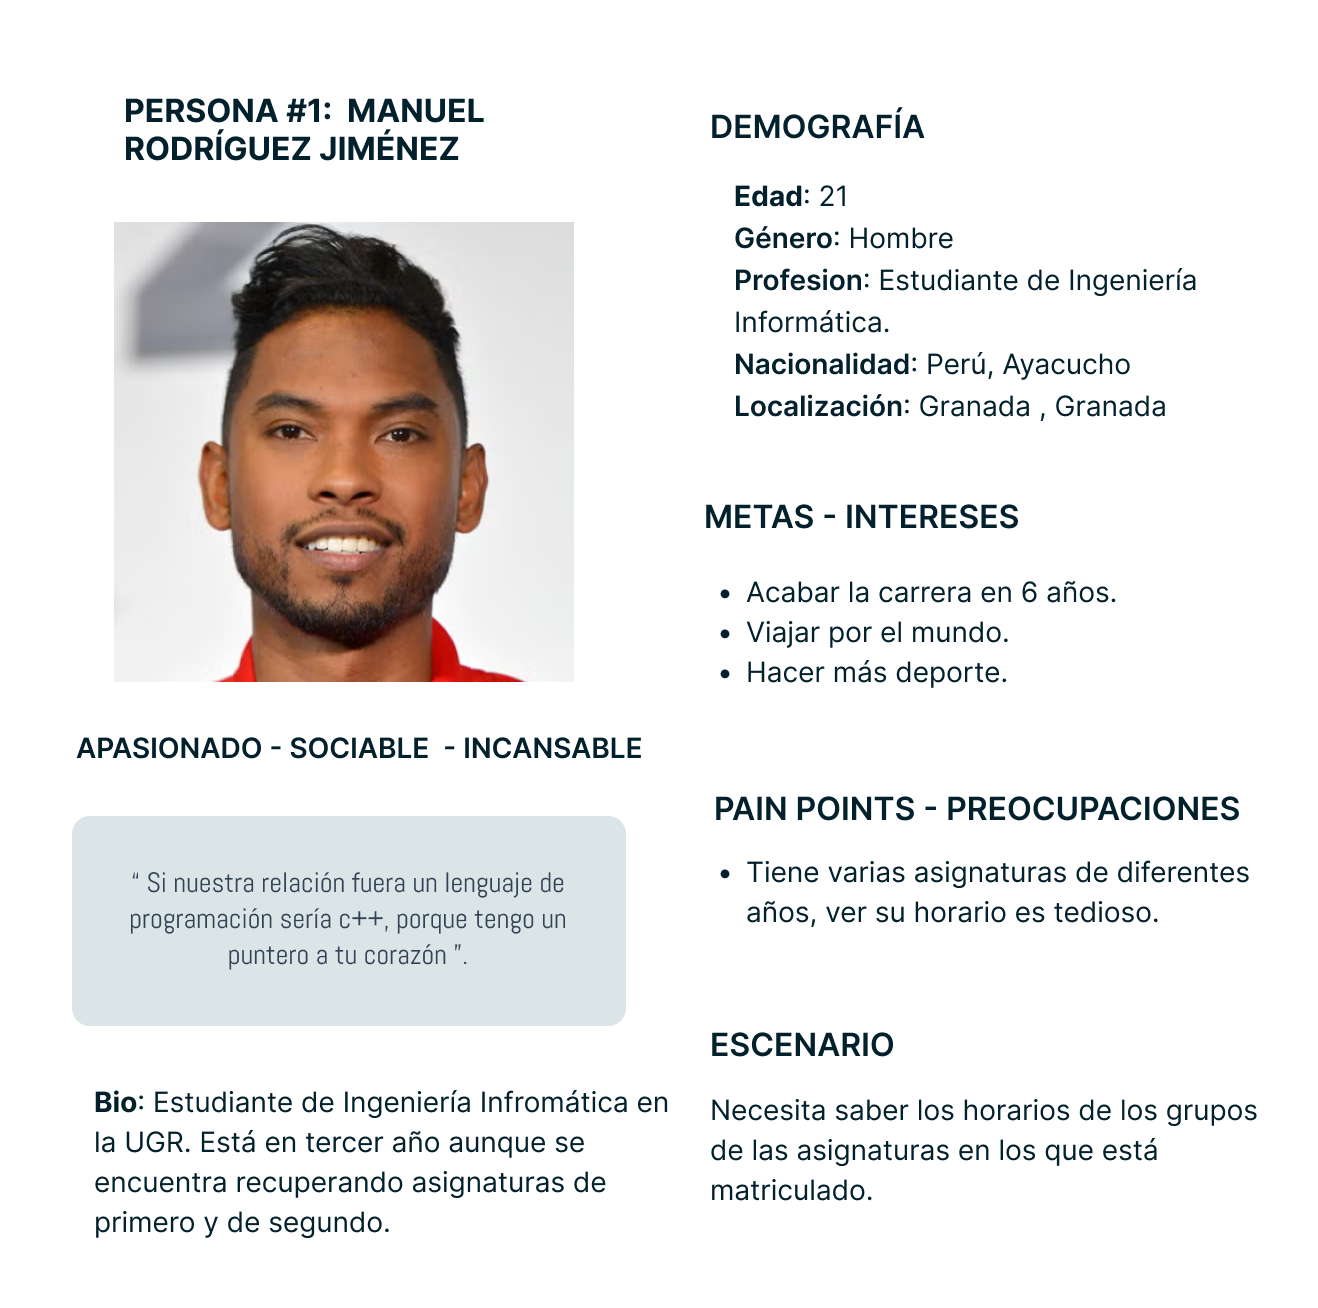
\includegraphics[width=0.6\textwidth]{figures/04_persona_1.png}
    \caption{Persona 1: Alumno de la UGR}
    \label{fig:persona_1}
\end{figure}

\begin{figure}[H]
    \centering
    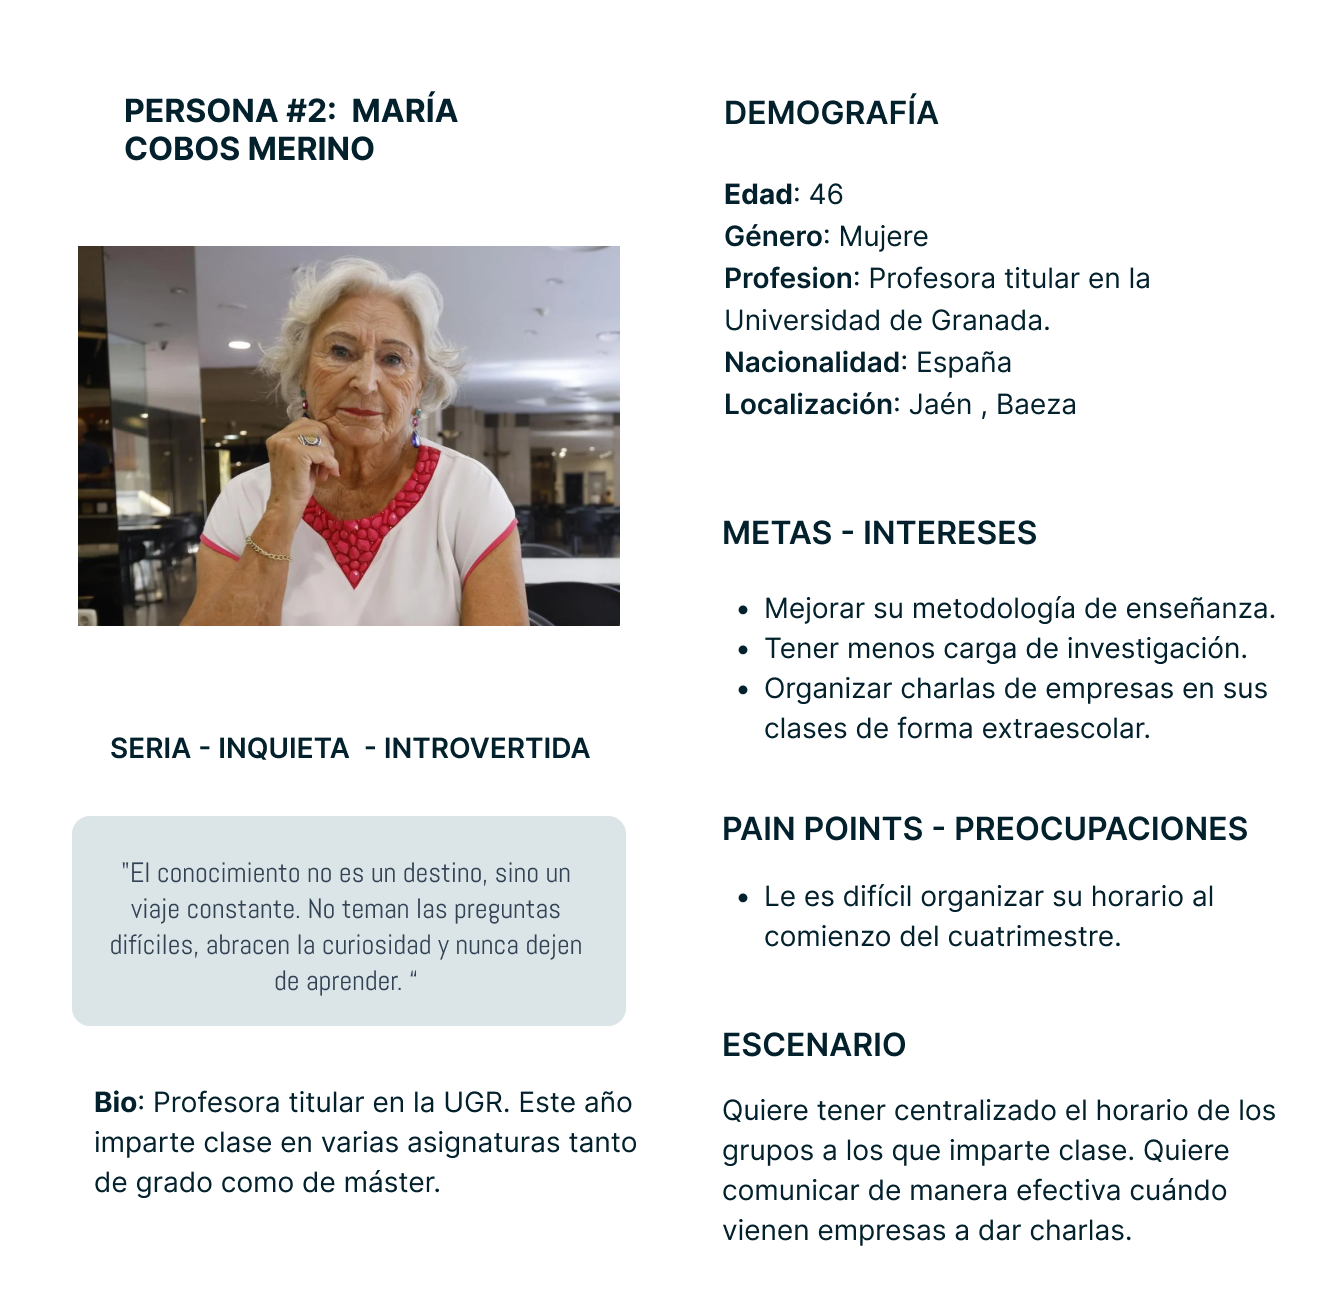
\includegraphics[width=0.6\textwidth]{figures/04_persona_2.png}
    \caption{Persona 2: Profesor de la UGR}
    \label{fig:persona_2}
\end{figure}

\begin{figure}[H]
    \centering
    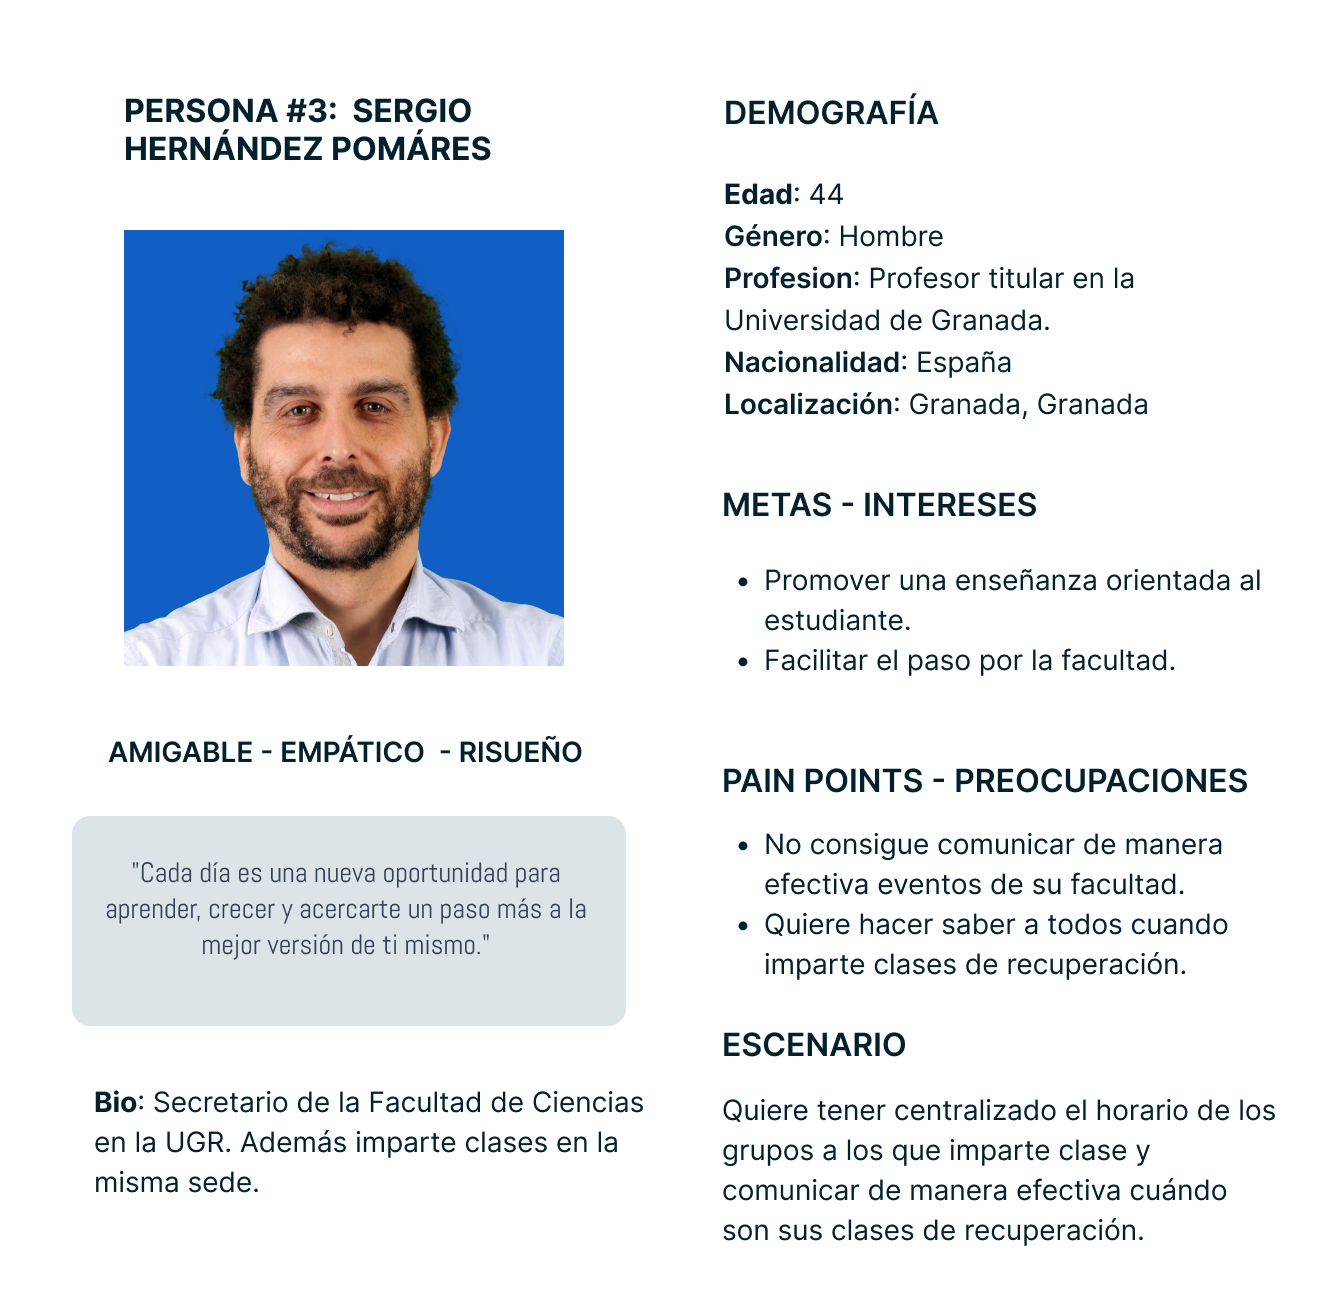
\includegraphics[width=0.6\textwidth]{figures/04_persona_3.png}
    \caption{Persona 3: ''Administrador'' de la UGR}
    \label{fig:persona_3}
\end{figure}

\section{Escenarios}

Un escenario es una descripción narrativa de cómo un usuario interactúa con un sistema para lograr un objetivo específico. Los escenarios son herramientas útiles para comprender y comunicar los requisitos del sistema, ya que proporcionan un contexto claro y detallado sobre cómo se espera que funcione el sistema en situaciones del mundo real.
\newline
\negritas{¿Por qué son importantes los escenarios?}
\begin{itemize}
    \item Ayudan a identificar y definir los requisitos del sistema de manera más clara y comprensible.
    \item Proporcionan un contexto para las decisiones de diseño y desarrollo, asegurando que se alineen con las necesidades del usuario.
    \item Facilitan la comunicación entre los miembros del equipo de desarrollo y los interesados, ya que son más fáciles de entender que los requisitos técnicos.
    \item Permiten identificar posibles problemas o desafíos en la interacción del usuario con el sistema antes de que se implemente.
\end{itemize}

\subsection{Escenarios del sistema}

\subsubsection*{Escenario 1: Manuel, el alumno organizado en medio del caos}

\textbf{Situación Actual:} Manuel es estudiante de tercer año del Grado de Química en la Facultad de Ciencias de la UGR. Este curso, su horario es un verdadero rompecabezas: tiene asignaturas de primero, segundo y tercero. Para complicar aún más las cosas, varios grupos han cambiado de aula a última hora. Manuel se encuentra constantemente revisando múltiples documentos, correos electrónicos y tablones de anuncios para intentar confeccionar un horario coherente y no perderse ninguna clase. La incertidumbre sobre dónde y cuándo tiene cada asignatura le genera estrés y dificulta su planificación semanal.

\textbf{Con el Sistema:} Manuel accede a su panel personalizado. Allí, visualiza de forma clara y unificada su horario, con todas las asignaturas de los diferentes cursos que tiene matriculadas. La información de las aulas está completamente actualizada, reflejando los últimos cambios. Además, puede filtrar por formato mensual, semanal y diario, facilitando la consulta. Con una url para importar en un sistema de calendario externo, sincroniza este horario personalizado con su Google Calendar, teniendo toda su planificación académica integrada en su calendario digital habitual. Ya no tiene que preocuparse por buscar información dispersa o por posibles cambios de última hora, ya que la aplicación se encarga de mantener su horario al día.

\subsubsection*{Escenario 2: María, la profesora conectada con sus alumnos}

\textbf{Situación Actual:} La profesora María imparte varias asignaturas en la UGR y utiliza el SWAD para comunicar anuncios importantes a sus alumnos, como clases de recuperación o charlas de profesionales invitados. Sin embargo, se da cuenta de que muchos estudiantes no acceden regularmente a la plataforma o no revisan los mensajes con la frecuencia necesaria, perdiéndose información valiosa. Para aquellos que sí ven el mensaje, recordar la fecha y hora del evento implica tener que buscarlo nuevamente en el SWAD. Esto dificulta la participación de los alumnos en actividades complementarias importantes para su formación.

\textbf{Con el Sistema:} María puede crear eventos directamente asociados a sus grupos de asignatura. Al hacerlo, el sistema automáticamente envía una notificación por correo electrónico a todos los alumnos inscritos en ese grupo, informándoles del evento con todos los detalles relevantes (fecha, hora, lugar, descripción). Además, este evento se añade automáticamente al calendario personal de cada alumno dentro de la aplicación, integrado con sus clases oficiales. María también puede sincronizar su propio calendario de eventos y clases con su Google Calendar, teniendo una visión completa de su agenda académica. De esta manera, la información importante llega directamente a los alumnos, aumentando la visibilidad y la participación en las actividades propuestas.

\subsubsection*{Escenario 3: Sergio, el administrador eficiente con información clara}

\textbf{Situación Actual:} Sergio, el secretario de la ETSIIT, necesita tener una visión clara del horario de clases que se imparten en la facultad para diversas tareas de gestión y organización. Además, la facultad organiza regularmente seminarios de empresas, talleres y otros eventos de interés para los estudiantes. Actualmente, la comunicación de estos eventos se realiza principalmente por correo electrónico masivo, lo que a menudo resulta intrusivo y puede pasar desapercibido entre la gran cantidad de mensajes que reciben los alumnos. Sergio necesita una forma más efectiva y menos invasiva de informar sobre estos eventos a nivel de facultad.

\textbf{Con el Sistema:} Sergio puede visualizar el horario de todas las clases de la ETSIIT de forma organizada y sencilla a través de la interfaz del sistema. Además, tiene la capacidad de crear eventos a nivel de facultad (seminarios, talleres, etc.). Estos eventos se integran directamente en el calendario de todos los alumnos de la ETSIIT dentro de la aplicación, apareciendo junto con sus horarios de clase habituales. Aunque no se envía una notificación por correo electrónico para evitar la sobrecarga de información, los alumnos pueden ver fácilmente estos eventos al consultar su horario personalizado. De esta manera, la información importante a nivel de facultad está siempre accesible y visible para los estudiantes, mejorando la comunicación y la participación sin recurrir a métodos intrusivos.

\section{Historias de usuario}

Una historia de usuario es una explicación general e informal de una función de software escrita desde la perspectiva
del usuario final. Su propósito es articular cómo proporcionará una función de software valor al cliente. \cite{atlassian_user_stories}.

Estas no usan un lenguaje técnico y preciso para definir y acotar los requisitos de un sistema, sino que se enfocan en
el usuario final y en cómo este interactuará con el sistema. Por lo tanto, las historias de usuario son una herramienta
de comunicación entre el equipo de desarrollo y el cliente.

En \hyperlink{scrum}{Scrum} las historias de usuario son una parte fundamental del proceso de desarrollo de software. En
este marco de trabajo, las historias de usuario son utilizadas para definir los requisitos del sistema y son la base para
la planificación y estimación de las tareas a realizar.
\newline\newline
\negritas{¿Por qué son importantes las historias de usuario?}
\begin{itemize}
    \item Centran la atención en el usuario final.
    \item Permiten la colaboración y comunicación entre el equipo de desarrollo y el cliente.
    \item Fomentan soluciones creativas y flexibles.
\end{itemize}
\subsection{Estructura de una historia de usuario}

Las historias de usuario siguen una estructura general simple y clara. 
\newline\newline
\textbf{Como} [tipo de usuario], \textbf{quiero} [realizar una acción], \textbf{para} [obtener un beneficio].

\begin{itemize}
    \item \textbf{Como}: describe el tipo de usuario que está interactuando con el sistema.
    \item \textbf{Quiero}: describe la acción que el usuario desea realizar.
    \item \textbf{Para}: describe el beneficio que el usuario obtendrá al realizar la acción.   
\end{itemize}

Además de esta estructura general, las historias de usuario pueden incluir otros elementos como criterios de aceptación,
prioridad, estimación de esfuerzo, entre otros.

Para se ha definido la siguiente estructura para las historias de usuario:

%% Tabla: Estructura de una historia de usuario
\begin{table}[H]
    \centering
    \begin{tabular}{|p{2cm}|p{4cm}|p{2cm}|p{4cm}|}
        \hline
        \textbf{ID} & Identificador único de la historia de usuario. & \textbf{Nombre} & Nombre de la historia de usuario. \\
        \hline
        \multicolumn{2}{|p{6cm}|}{\textbf{Descripción}} & \multicolumn{2}{p{6cm}|}{Descripción general de la historia de usuario.} \\
        \hline
        \multicolumn{2}{|p{6cm}|}{\textbf{Estimación}} & \multicolumn{2}{p{6cm}|}{Estimación del esfuerzo necesario para completar la historia de usuario. Basado en Planning Poker.} \\
        \hline
        \multicolumn{2}{|p{6cm}|}{\textbf{Prioridad}} & \multicolumn{2}{p{6cm}|}{Acción que el usuario desea realizar. Desde P3 (baja) hasta P0 (alta).} \\
        \hline
        \multicolumn{2}{|p{6cm}|}{\textbf{Criterios de aceptación}} & \multicolumn{2}{p{6cm}|}{Conjunto de condiciones que deben cumplirse para considerar la historia de usuario como completada.} \\
        \hline
    \end{tabular}
    \caption{Estructura de una historia de usuario}
    \label{tab:estructura_historia_usuario}
\end{table}

\subsection{Historias de usuario}

\begin{table}[H]
    \centering
    \begin{tabular}{|p{2cm}|p{4cm}|p{2cm}|p{4cm}|}
        \hline
        \textbf{ID} & HU-1 & \textbf{Nombre} & Iniciar sesión \\
        \hline
        \multicolumn{2}{|p{6cm}|}{\textbf{Descripción}} & \multicolumn{2}{p{6cm}|}{Como usuario he de poder iniciar sesión en el sistema.} \\
        \hline
        \multicolumn{2}{|p{6cm}|}{\textbf{Estimación}} & \multicolumn{2}{p{6cm}|}{3} \\
        \hline
        \multicolumn{2}{|p{6cm}|}{\textbf{Prioridad}} & \multicolumn{2}{p{6cm}|}{P0} \\
        \hline
        \multicolumn{2}{|p{6cm}|}{\textbf{Criterios de aceptación}} & \multicolumn{2}{p{6cm}|}{
            \begin{itemize}
                \item Para poder iniciar sesión ha de insertar su correo y contraseña.
                \item Sólo se puede iniciar sesión con correos de la UGR.
            \end{itemize}
        } \\
        \hline
    \end{tabular}
    \caption{Historia de usuario HU-1}
    \label{tab:hu_1}
\end{table}

\begin{table}[H]
    \centering
    \begin{tabular}{|p{2cm}|p{4cm}|p{2cm}|p{4cm}|}
        \hline
        \textbf{ID} & HU-2 & \textbf{Nombre} & Registrarse \\
        \hline
        \multicolumn{2}{|p{6cm}|}{\textbf{Descripción}} & \multicolumn{2}{p{6cm}|}{Como usuario he de poder registrarme en el sistema.} \\
        \hline
        \multicolumn{2}{|p{6cm}|}{\textbf{Estimación}} & \multicolumn{2}{p{6cm}|}{5} \\
        \hline
        \multicolumn{2}{|p{6cm}|}{\textbf{Prioridad}} & \multicolumn{2}{p{6cm}|}{P0} \\
        \hline
        \multicolumn{2}{|p{6cm}|}{\textbf{Criterios de aceptación}} & \multicolumn{2}{p{6cm}|}{
            \begin{itemize}
                \item El alumno sólo se puede registrar con su correo institucional de la UGR.
                \item El alumno debe insertar nickname, correo y contraseña.
                \item La contraseña del alumno ha de ser mayor o igual a 9 caracteres, conteniendo esta una mayúscula y un número como mínimo.
                \item El registro se ha de completar mediante un link mandado por mail.
            \end{itemize}
        } \\
        \hline
    \end{tabular}
    \caption{Historia de usuario HU-2}
    \label{tab:hu_2}
\end{table}

\begin{table}[H]
    \centering
    \begin{tabular}{|p{2cm}|p{4cm}|p{2cm}|p{4cm}|}
        \hline
        \textbf{ID} & HU-3 & \textbf{Nombre} & Modificar nickname \\
        \hline
        \multicolumn{2}{|p{6cm}|}{\textbf{Descripción}} & \multicolumn{2}{p{6cm}|}{Como usuario puedo modificar mi nickname.} \\
        \hline
        \multicolumn{2}{|p{6cm}|}{\textbf{Estimación}} & \multicolumn{2}{p{6cm}|}{2} \\
        \hline
        \multicolumn{2}{|p{6cm}|}{\textbf{Prioridad}} & \multicolumn{2}{p{6cm}|}{P2} \\
        \hline
        \multicolumn{2}{|p{6cm}|}{\textbf{Criterios de aceptación}} & \multicolumn{2}{p{6cm}|}{
            \begin{itemize}
                \item El alumno no puede cambiar su nickname a otro que exista.
                \item El alumno no puede modificar su correo electrónico.
            \end{itemize}
        } \\
        \hline
    \end{tabular}
    \caption{Historia de usuario HU-3}
    \label{tab:hu_3}
\end{table}

\begin{table}[H]
    \centering
    \begin{tabular}{|p{2cm}|p{4cm}|p{2cm}|p{4cm}|}
        \hline
        \textbf{ID} & HU-4 & \textbf{Nombre} & Modificar contraseña \\
        \hline
        \multicolumn{2}{|p{6cm}|}{\textbf{Descripción}} & \multicolumn{2}{p{6cm}|}{Como usuario he de poder modificar la contraseña de acceso.} \\
        \hline
        \multicolumn{2}{|p{6cm}|}{\textbf{Estimación}} & \multicolumn{2}{p{6cm}|}{3} \\
        \hline
        \multicolumn{2}{|p{6cm}|}{\textbf{Prioridad}} & \multicolumn{2}{p{6cm}|}{P1} \\
        \hline
        \multicolumn{2}{|p{6cm}|}{\textbf{Criterios de aceptación}} & \multicolumn{2}{p{6cm}|}{
            \begin{itemize}
                \item Para poder modificar la contraseña ha de insertar la contraseña anterior.
                \item Se ha de insertar la nueva contraseña 2 veces, siendo esta  mayor o igual a 9 caracteres, y conteniendo una mayúscula y un número como mínimo.
            \end{itemize}
        } \\
        \hline
    \end{tabular}
    \caption{Historia de usuario HU-4}
    \label{tab:hu_4}
\end{table}

\begin{table}[H]
    \centering
    \begin{tabular}{|p{2cm}|p{4cm}|p{2cm}|p{4cm}|}
        \hline
        \textbf{ID} & HU-5 & \textbf{Nombre} & Darse de baja \\
        \hline
        \multicolumn{2}{|p{6cm}|}{\textbf{Descripción}} & \multicolumn{2}{p{6cm}|}{Como usuario
        he de poder darme de baja del sistema.} \\
        \hline
        \multicolumn{2}{|p{6cm}|}{\textbf{Estimación}} & \multicolumn{2}{p{6cm}|}{1} \\
        \hline
        \multicolumn{2}{|p{6cm}|}{\textbf{Prioridad}} & \multicolumn{2}{p{6cm}|}{P2} \\
        \hline
        \multicolumn{2}{|p{6cm}|}{\textbf{Criterios de aceptación}} & \multicolumn{2}{p{6cm}|}{
            \begin{itemize}
                \item Para poder completar la baja ha de escribir su contraseña en un campo de texto.
            \end{itemize}
        } \\
        \hline
    \end{tabular}
    \caption{Historia de usuario HU-5}
    \label{tab:hu_5}
\end{table}

\begin{table}[H]
    \centering
    \begin{tabular}{|p{2cm}|p{4cm}|p{2cm}|p{4cm}|}
        \hline
        \textbf{ID} & HU-6 & \textbf{Nombre} & Cambiar rol \\
        \hline
        \multicolumn{2}{|p{6cm}|}{\textbf{Descripción}} & \multicolumn{2}{p{6cm}|}{Como administrador he de poder actualizar mi rol a profesor, y viceversa.} \\
        \hline
        \multicolumn{2}{|p{6cm}|}{\textbf{Estimación}} & \multicolumn{2}{p{6cm}|}{2} \\
        \hline
        \multicolumn{2}{|p{6cm}|}{\textbf{Prioridad}} & \multicolumn{2}{p{6cm}|}{P1} \\
        \hline
        \multicolumn{2}{|p{6cm}|}{\textbf{Criterios de aceptación}} & \multicolumn{2}{p{6cm}|}{
            \begin{itemize}
                \item Para poder cambiar el rol a profesor he de ser administrador.
                \item Para poder cambiar el rol a profesor he de ser administrador.
            \end{itemize}
        } \\
        \hline
    \end{tabular}
    \caption{Historia de usuario HU-6}
    \label{tab:hu_6}
\end{table}

\begin{table}[H]
    \centering
    \begin{tabular}{|p{2cm}|p{4cm}|p{2cm}|p{4cm}|}
        \hline
        \textbf{ID} & HU-7 & \textbf{Nombre} & Seleccionar grados \\
        \hline
        \multicolumn{2}{|p{6cm}|}{\textbf{Descripción}} & \multicolumn{2}{p{6cm}|}{Como usuario he de poder seleccionar el grado o grados que estoy cursando.} \\
        \hline
        \multicolumn{2}{|p{6cm}|}{\textbf{Estimación}} & \multicolumn{2}{p{6cm}|}{3} \\
        \hline
        \multicolumn{2}{|p{6cm}|}{\textbf{Prioridad}} & \multicolumn{2}{p{6cm}|}{P0} \\
        \hline
        \multicolumn{2}{|p{6cm}|}{\textbf{Criterios de aceptación}} & \multicolumn{2}{p{6cm}|}{
            \begin{itemize}
                \item Se pueden seleccionar un máximo de 4 grados.
            \end{itemize}
        } \\
        \hline
    \end{tabular}
    \caption{Historia de usuario HU-7}
    \label{tab:hu_7}
\end{table}

\begin{table}[H]
    \centering
    \begin{tabular}{|p{2cm}|p{4cm}|p{2cm}|p{4cm}|}
        \hline
        \textbf{ID} & HU-8 & \textbf{Nombre} & Eliminar grado \\
        \hline
        \multicolumn{2}{|p{6cm}|}{\textbf{Descripción}} & \multicolumn{2}{p{6cm}|}{Como usuario he de poder eliminar un grado que ya no esté cursando.} \\
        \hline
        \multicolumn{2}{|p{6cm}|}{\textbf{Estimación}} & \multicolumn{2}{p{6cm}|}{2} \\
        \hline
        \multicolumn{2}{|p{6cm}|}{\textbf{Prioridad}} & \multicolumn{2}{p{6cm}|}{P1} \\
        \hline
        \multicolumn{2}{|p{6cm}|}{\textbf{Criterios de aceptación}} & \multicolumn{2}{p{6cm}|}{
            \begin{itemize}
                \item Si el usuario está suscrito a grupos de asignatura de ese grado, se le recordará que también se revocarán sus suscripciones a estos.
            \end{itemize}
        } \\
        \hline
    \end{tabular}
    \caption{Historia de usuario HU-8}
    \label{tab:hu_8}
\end{table}

\begin{table}[H]
    \centering
    \begin{tabular}{|p{2cm}|p{4cm}|p{2cm}|p{4cm}|}
        \hline
        \textbf{ID} & HU-9 & \textbf{Nombre} & Suscribirse a grupos de asignatura \\
        \hline
        \multicolumn{2}{|p{6cm}|}{\textbf{Descripción}} & \multicolumn{2}{p{6cm}|}{Como usuario he de poder suscribirme a los grupos de asignaturas a las que quiero hacer seguimiento.} \\
        \hline
        \multicolumn{2}{|p{6cm}|}{\textbf{Estimación}} & \multicolumn{2}{p{6cm}|}{4} \\
        \hline
        \multicolumn{2}{|p{6cm}|}{\textbf{Prioridad}} & \multicolumn{2}{p{6cm}|}{P0} \\
        \hline
        \multicolumn{2}{|p{6cm}|}{\textbf{Criterios de aceptación}} & \multicolumn{2}{p{6cm}|}{
            \begin{itemize}
                \item Para hacer seguimiento a un grupo en concreto, el usuario deberá estar cursando el grado al que pertenece.
            \end{itemize}
        } \\
        \hline
    \end{tabular}
    \caption{Historia de usuario HU-9}
    \label{tab:hu_9}
\end{table}

\begin{table}[H]
    \centering
    \begin{tabular}{|p{2cm}|p{4cm}|p{2cm}|p{4cm}|}
        \hline
        \textbf{ID} & HU-10 & \textbf{Nombre} & Revocar suscripción a grupo de asignatura \\
        \hline
        \multicolumn{2}{|p{6cm}|}{\textbf{Descripción}} & \multicolumn{2}{p{6cm}|}{Como usuario he de poder revocar una suscripción a un grupo de asignatura.} \\
        \hline
        \multicolumn{2}{|p{6cm}|}{\textbf{Estimación}} & \multicolumn{2}{p{6cm}|}{2} \\
        \hline
        \multicolumn{2}{|p{6cm}|}{\textbf{Prioridad}} & \multicolumn{2}{p{6cm}|}{P1} \\
        \hline
        \multicolumn{2}{|p{6cm}|}{\textbf{Criterios de aceptación}} & \multicolumn{2}{p{6cm}|}{
            \begin{itemize}
                \item El usuario sólo puede revocar suscripciones de grupos a los que está suscrito.
            \end{itemize}
        } \\
        \hline
    \end{tabular}
    \caption{Historia de usuario HU-10}
    \label{tab:hu_10}
\end{table}

\begin{table}[H]
    \centering
    \begin{tabular}{|p{2cm}|p{4cm}|p{2cm}|p{4cm}|}
        \hline
        \textbf{ID} & HU-11 & \textbf{Nombre} & Ver horario de grupos de asignatura \\
        \hline
        \multicolumn{2}{|p{6cm}|}{\textbf{Descripción}} & \multicolumn{2}{p{6cm}|}{Como usuario he de poder obtener la información de mi horario personalizado conforme a las suscripciones.} \\
        \hline
        \multicolumn{2}{|p{6cm}|}{\textbf{Estimación}} & \multicolumn{2}{p{6cm}|}{5} \\
        \hline
        \multicolumn{2}{|p{6cm}|}{\textbf{Prioridad}} & \multicolumn{2}{p{6cm}|}{P0} \\
        \hline
        \multicolumn{2}{|p{6cm}|}{\textbf{Criterios de aceptación}} & \multicolumn{2}{p{6cm}|}{
            \begin{itemize}
                \item El horario de cada clase debe mostrar la asignatura, grupo, hora de inicio y fin, profesores del grupo, y aula.
                \item Las clases sólo deben mostrarse en el rango de fechas en las que se imparten.
            \end{itemize}
        } \\
        \hline
    \end{tabular}
    \caption{Historia de usuario HU-11}
    \label{tab:hu_11}
\end{table}

\begin{table}[H]
    \centering
    \begin{tabular}{|p{2cm}|p{4cm}|p{2cm}|p{4cm}|}
        \hline
        \textbf{ID} & HU-12 & \textbf{Nombre} & Crear evento puntual a nivel de grupo de asignatura \\
        \hline
        \multicolumn{2}{|p{6cm}|}{\textbf{Descripción}} & \multicolumn{2}{p{6cm}|}{Como profesor / administrador he de poder crear eventos puntuales a nivel de grupo ( clases de recuperación, extra, charlas …).} \\
        \hline
        \multicolumn{2}{|p{6cm}|}{\textbf{Estimación}} & \multicolumn{2}{p{6cm}|}{3} \\
        \hline
        \multicolumn{2}{|p{6cm}|}{\textbf{Prioridad}} & \multicolumn{2}{p{6cm}|}{P0} \\
        \hline
        \multicolumn{2}{|p{6cm}|}{\textbf{Criterios de aceptación}} & \multicolumn{2}{p{6cm}|}{
            \begin{itemize}
                \item Se debe especificar la fecha, hora de inicio, hora de fin y tipo de evento.
                \item La clase extra no debe coincidir con otra clase existente en horario y aula.
                \item El usuario debe ser un profesor o administrador.
            \end{itemize}
        } \\
        \hline
    \end{tabular}
    \caption{Historia de usuario HU-12}
    \label{tab:hu_12}
\end{table}

\begin{table}[H]
    \centering
    \begin{tabular}{|p{2cm}|p{4cm}|p{2cm}|p{4cm}|}
        \hline
        \textbf{ID} & HU-13 & \textbf{Nombre} & Eliminar evento puntual a nivel de grupo de asignatura \\
        \hline
        \multicolumn{2}{|p{6cm}|}{\textbf{Descripción}} & \multicolumn{2}{p{6cm}|}{Como profesor / administrador he de poder eliminar los eventos que he creado ( clases de recuperación, extra, charlas …).} \\
        \hline
        \multicolumn{2}{|p{6cm}|}{\textbf{Estimación}} & \multicolumn{2}{p{6cm}|}{2} \\
        \hline
        \multicolumn{2}{|p{6cm}|}{\textbf{Prioridad}} & \multicolumn{2}{p{6cm}|}{P1} \\
        \hline
        \multicolumn{2}{|p{6cm}|}{\textbf{Criterios de aceptación}} & \multicolumn{2}{p{6cm}|}{
            \begin{itemize}
                \item Se debe especificar la fecha, hora de inicio, hora de fin y tipo de evento.
                \item La clase extra no debe coincidir con otra clase existente en horario y aula.
                \item El usuario debe ser un profesor o administrador.
            \end{itemize}
        } \\
        \hline
    \end{tabular}
    \caption{Historia de usuario HU-13}
    \label{tab:hu_13}
\end{table}

\begin{table}[H]
    \centering
    \begin{tabular}{|p{2cm}|p{4cm}|p{2cm}|p{4cm}|}
        \hline
        \textbf{ID} & HU-14 & \textbf{Nombre} & Exportar horario a calendario estándar \\
        \hline
        \multicolumn{2}{|p{6cm}|}{\textbf{Descripción}} & \multicolumn{2}{p{6cm}|}{Como usuario he de poder exportar mi horario para usarlo en otros sistemas estándar de calendario.} \\
        \hline
        \multicolumn{2}{|p{6cm}|}{\textbf{Estimación}} & \multicolumn{2}{p{6cm}|}{4} \\
        \hline
        \multicolumn{2}{|p{6cm}|}{\textbf{Prioridad}} & \multicolumn{2}{p{6cm}|}{P0} \\
        \hline
        \multicolumn{2}{|p{6cm}|}{\textbf{Criterios de aceptación}} & \multicolumn{2}{p{6cm}|}{
            \begin{itemize}
                \item El usuario podrá exportar su horario en formatos compatibles con sistemas estándar de calendario (.ics).
                \item La exportación debe incluir todas las asignaturas y eventos del usuario.
                \item Se debe permitir elegir un rango de fechas para la exportación.
                \item El archivo generado debe poder descargarse y ser importable en Google Calendar, Outlook, Apple Calendar, etc.
            \end{itemize}
        } \\
        \hline
    \end{tabular}
    \caption{Historia de usuario HU-14}
    \label{tab:hu_14}
\end{table}

\begin{table}[H]
    \centering
    \begin{tabular}{|p{2cm}|p{4cm}|p{2cm}|p{4cm}|}
        \hline
        \textbf{ID} & HU-15 & \textbf{Nombre} & Sincronizar calendario con Google Calendar \\
        \hline
        \multicolumn{2}{|p{6cm}|}{\textbf{Descripción}} & \multicolumn{2}{p{6cm}|}{Como usuario he de poder sincronizar mi calendario con Google Calendar.} \\
        \hline
        \multicolumn{2}{|p{6cm}|}{\textbf{Estimación}} & \multicolumn{2}{p{6cm}|}{5} \\
        \hline
        \multicolumn{2}{|p{6cm}|}{\textbf{Prioridad}} & \multicolumn{2}{p{6cm}|}{P3} \\
        \hline
        \multicolumn{2}{|p{6cm}|}{\textbf{Criterios de aceptación}} & \multicolumn{2}{p{6cm}|}{
            \begin{itemize}
                \item El usuario podrá vincular su cuenta con Google Calendar mediante OAuth.
                \item Los eventos de su horario deben sincronizarse automáticamente con Google Calendar.
                \item Se deben reflejar en Google Calendar los cambios realizados en el horario del usuario.
                \item El usuario debe poder desactivar la sincronización en cualquier momento.
            \end{itemize}
        } \\
        \hline
    \end{tabular}
    \caption{Historia de usuario HU-15}
    \label{tab:hu_15}
\end{table}

\begin{table}[H]
    \centering
    \begin{tabular}{|p{2cm}|p{4cm}|p{2cm}|p{4cm}|}
        \hline
        \textbf{ID} & HU-16 & \textbf{Nombre} & Ver alertas de clases extra de grupos de asignatura \\
        \hline
        \multicolumn{2}{|p{6cm}|}{\textbf{Descripción}} & \multicolumn{2}{p{6cm}|}{Como alumno he de poder recibir alertas referentes a “clases extra” de mis grupos ( clases de recuperación, extra, charlas …).} \\
        \hline
        \multicolumn{2}{|p{6cm}|}{\textbf{Estimación}} & \multicolumn{2}{p{6cm}|}{3} \\
        \hline
        \multicolumn{2}{|p{6cm}|}{\textbf{Prioridad}} & \multicolumn{2}{p{6cm}|}{P1} \\
        \hline
        \multicolumn{2}{|p{6cm}|}{\textbf{Criterios de aceptación}} & \multicolumn{2}{p{6cm}|}{
            \begin{itemize}
                \item Las clases extra aparecerán, como las clases, en la vista del horario.
                \item Si el evento es en la semana actual se debe mostrar en una lista de alertas.
                \item Se debe mandar un correo electrónico a los alumnos que afecte y tengan las notificaciones activadas.
            \end{itemize}
        } \\
        \hline
    \end{tabular}
    \caption{Historia de usuario HU-16}
    \label{tab:hu_16}
\end{table}

\begin{table}[H]
    \centering
    \begin{tabular}{|p{2cm}|p{4cm}|p{2cm}|p{4cm}|}
        \hline
        \textbf{ID} & HU-17 & \textbf{Nombre} & Crear evento a nivel de facultad \\
        \hline
        \multicolumn{2}{|p{6cm}|}{\textbf{Descripción}} & \multicolumn{2}{p{6cm}|}{Como administrador he de poder crear eventos a nivel de facultad ( charlas, conferencias, exámenes …).} \\
        \hline
        \multicolumn{2}{|p{6cm}|}{\textbf{Estimación}} & \multicolumn{2}{p{6cm}|}{5} \\
        \hline
        \multicolumn{2}{|p{6cm}|}{\textbf{Prioridad}} & \multicolumn{2}{p{6cm}|}{P1} \\
        \hline
        \multicolumn{2}{|p{6cm}|}{\textbf{Criterios de aceptación}} & \multicolumn{2}{p{6cm}|}{
            \begin{itemize}
                \item Se debe especificar la fecha, hora de inicio, hora de fin y tipo de evento.
                \item El evento no debe coincidir con otra clase existente en horario y aula.
                \item El usuario debe ser un administrador.
            \end{itemize}
        } \\
        \hline
    \end{tabular}
    \caption{Historia de usuario HU-17}
    \label{tab:hu_17}
\end{table}

\begin{table}[H]
    \centering
    \begin{tabular}{|p{2cm}|p{4cm}|p{2cm}|p{4cm}|}
        \hline
        \textbf{ID} & HU-18 & \textbf{Nombre} & Eliminar evento a nivel de facultad \\
        \hline
        \multicolumn{2}{|p{6cm}|}{\textbf{Descripción}} & \multicolumn{2}{p{6cm}|}{Como profesor / administrador he de poder eliminar los eventos que he creado a nivel de facultad ( charlas, conferencias, exámenes …).} \\
        \hline
        \multicolumn{2}{|p{6cm}|}{\textbf{Estimación}} & \multicolumn{2}{p{6cm}|}{3} \\
        \hline
        \multicolumn{2}{|p{6cm}|}{\textbf{Prioridad}} & \multicolumn{2}{p{6cm}|}{P2} \\
        \hline
        \multicolumn{2}{|p{6cm}|}{\textbf{Criterios de aceptación}} & \multicolumn{2}{p{6cm}|}{
            \begin{itemize}
                \item El usuario debe ser un administrador.
            \end{itemize}
        } \\
        \hline
    \end{tabular}
    \caption{Historia de usuario HU-18}
    \label{tab:hu_18}
\end{table}

\begin{table}[H]
    \centering
    \begin{tabular}{|p{2cm}|p{4cm}|p{2cm}|p{4cm}|}
        \hline
        \textbf{ID} & HU-19 & \textbf{Nombre} & Activar / desactivar alertas por correo electrónico \\
        \hline
        \multicolumn{2}{|p{6cm}|}{\textbf{Descripción}} & \multicolumn{2}{p{6cm}|}{Como alumno debo poder desactivar / activar las notificaciones por correo electrónico referente a los eventos a nivel de grupo / facultad} \\
        \hline
        \multicolumn{2}{|p{6cm}|}{\textbf{Estimación}} & \multicolumn{2}{p{6cm}|}{3} \\
        \hline
        \multicolumn{2}{|p{6cm}|}{\textbf{Prioridad}} & \multicolumn{2}{p{6cm}|}{P2} \\
        \hline
        \multicolumn{2}{|p{6cm}|}{\textbf{Criterios de aceptación}} & \multicolumn{2}{p{6cm}|}{
            \begin{itemize}
                \item Tras desactivar las alertas, el usuario no recibirá más correos electrónicos referente a eventos a nivel de grupo / facultad.
                \item El usuario podrá activar las alertas en cualquier momento.
            \end{itemize}
        } \\
        \hline
    \end{tabular}
    \caption{Historia de usuario HU-19}
    \label{tab:hu_19}
\end{table}

\begin{table}[H]
    \centering
    \begin{tabular}{|p{2cm}|p{4cm}|p{2cm}|p{4cm}|}
        \hline
        \textbf{ID} & HU-20 & \textbf{Nombre} & Suscripción a todas las asignaturas que imparte un profesor \\
        \hline
        \multicolumn{2}{|p{6cm}|}{\textbf{Descripción}} & \multicolumn{2}{p{6cm}|}{Como profesor he de poder buscar mi nombre, y aceptar suscribirme a las asignaturas a las que imparto clase en la UGR} \\
        \hline
        \multicolumn{2}{|p{6cm}|}{\textbf{Estimación}} & \multicolumn{2}{p{6cm}|}{5} \\
        \hline
        \multicolumn{2}{|p{6cm}|}{\textbf{Prioridad}} & \multicolumn{2}{p{6cm}|}{P2} \\
        \hline
        \multicolumn{2}{|p{6cm}|}{\textbf{Criterios de aceptación}} & \multicolumn{2}{p{6cm}|}{
            \begin{itemize}
                \item El nombre a buscar debe ser un profesor reflejado en la web Grados UGR.
                \item El usuario se suscribirá a todas las asignaturas que imparte el profesor.
            \end{itemize}
        } \\
        \hline
    \end{tabular}
    \caption{Historia de usuario HU-20}
    \label{tab:hu_20}
\end{table}


\section{Requisitos funcionales}

A partir de las historias de usuario, junto a sus criterios de aceptación, se han extraído los siguientes requisitos funcionales:

\subsection{Gestión de usuarios}

\begin{itemize}
    \item \textbf{RF-1) Gestión de usuarios:} El sistema debe poder registrar usuarios para futuros inicio de sesión y seguimiento de su información de suscripciones a grupos de asignaturas.
    \begin{itemize}
        \item \textbf{RF-1.1) Inicio de sesión:} El sistema debe permitir el inicio de sesión de usuarios mediante correo electrónico institucional y contraseña.
        \item \textbf{RF-2.2) Registro de usuarios:} El sistema debe tener un proceso de registro de usuario.
        \item \textbf{RF-2.3) Completar el registro:} Para completar el registro el sistema debe mandar un mail para confirmar si el usuario se trata de un alumno o de un profesor.
        \item \textbf{RF-2.4) Cambio de nickname:} El sistema debe permitir cambiar el nickname al usuario por uno no usado.
        \item \textbf{RF-2.5) Cambio de contraseña de acceso:} El sistema debe permitir el cambio de la contraseña de acceso.
        \item \textbf{RF-2.6) Dar de baja:} El sistema debe permitir al usuario darse de baja con el objetivo de que no le lleguen más correos relacionados.
        \item \textbf{RF-2.7) Cambio de rol:} EL sistema debe poder facilitar el cambio de rol de profesor a administrador, y viceversa.
        \item \textbf{RF-2.8) Activación / desactivación de alertas:} El sistema debe permitir activar o desactivar las alertas por correo electrónico.
        \item \textbf{RF-2.9) Suscripción a los grupos que imparte un profesor:} El sistema debe permitir al profesor suscribirse a los grupos de asignaturas que imparte.
    \end{itemize}
\end{itemize}

\subsection{Gestión de horarios académicos}

\begin{itemize}
    \item \textbf{RF-2) Gestión de horarios académicos:} El sistema debe poder obtener la información relacionada con el horario académico de todos los grados de la UGR, para así poder identificar los horarios personalizados de alumnos y docentes a través de un sistema de suscripción a grupos de asignatura.
    \begin{itemize}
        \item \textbf{RF-2.1) Recopilación de horarios:} El sistema debe recopilar la información de horarios académicos de todos los grados de la UGR.
        \item \textbf{RF-2.2) Grados del alumno / profesor:} El sistema debe recoger el grado/ grados académicos que está cursando / impartiendo el alumno / profesor.
        \item \textbf{RF-2.3) Asignaturas del alumno / profesor:} El sistema debe recoger las asignaturas que está cursando / impartiendo el alumno / profesor.
        \item \textbf{RF-2.4) Grupos del alumno / profesor:} El sistema debe recoger los grupos de las asignaturas que está cursando / impartiendo el alumno / profesor.
        \item \textbf{RF-2.5) Eliminar grados del alumno / profesor:} El sistema debe poder eliminar el grado/ grados académicos que está cursando / impartiendo el alumno / profesor.
        \item \textbf{RF-2.6) Eliminar asignaturas del alumno / profesor:} El sistema debe poder eliminar las asignaturas que está cursando / impartiendo el alumno / profesor.
        \item \textbf{RF-2.7) Eliminar grupos del alumno / profesor:} El sistema debe poder eliminar los grupos de las asignaturas que está cursando / impartiendo el alumno / profesor.
        \item \textbf{RF-2.8) Horario personalizado:} El usuario ha de poder acceder a la información de horario académico de los grupos de asignaturas a los que esté suscrito.
        \item \textbf{RF-2.9) Crear clases extra:} El sistema debe permitir al profesor / administrador crear clases extra a las oficiales.
        \item \textbf{RF-2.10) Eliminar clases extra:} El sistema debe permitir al profesor / administrador eliminar clases extra a las oficiales.
        \item \textbf{RF-2.11) Exportar horario a estándar:} El sistema debe poder exportar el horario en formato estándar (.ics).
        \item \textbf{RF-2.12) Sincronizar con Google calendar:} El sistema deberá poder sincronizarse con Google Calendar.
        \item \textbf{RF-2.13) Alertas sobre clases extra:} El sistema debe poder mandar alertas sobre clases extra a los alumnos de ese grupo.
        \item \textbf{RF-2.14) Crear eventos a nivel de facultad:} El sistema debe poder crear eventos a nivel de facultad.
        \item \textbf{RF-2.15) Alertas de cambios en asignaturas suscritas:} El sistema debe poder mandar alertas de cambios en las asignaturas suscritas.
        \item \textbf{RF-2.16) Eliminar eventos a nivel de facultad:} El sistema debe poder eliminar eventos a nivel de facultad.
    \end{itemize}
\end{itemize}

\section{Requisitos no funcionales}

\subsection{Rendimiento}

\begin{itemize}
    \item \textbf{RNF-1.1) Tiempo de respuesta:} El sistema debe responder a las solicitudes de los usuarios en un tiempo máximo de 2 segundos.
    \item \textbf{RNF-1.2) Capacidad de usuarios concurrentes:} El sistema debe soportar un mínimo de 1000 usuarios concurrentes sin degradación significativa del rendimiento.    \item \textbf{RNF-1.3) Recuperación ante fallos:} El sistema debe ser capaz de recuperarse de fallos en menos de 5 minutos.
\end{itemize}

\subsection{Usabilidad}

\begin{itemize}
    \item \textbf{RNF-2.1) Interfaz intuitiva:} La interfaz de usuario debe ser fácil de usar y comprender, incluso para usuarios sin experiencia técnica.
    \item \textbf{RNF-2.2) Accesibilidad:} El sistema debe cumplir con las pautas de accesibilidad web (WCAG) para garantizar que sea utilizable por personas con discapacidades.
    \item \textbf{RNF-2.3) Compatibilidad con dispositivos:} El sistema debe ser compatible con cualquier navegador web, y a cualquier resolución.
\end{itemize}

\subsection{Seguridad}

\begin{itemize}
    \item \textbf{RNF-3.1) Autenticación segura:} El sistema debe implementar un mecanismo de autenticación y autorización basado en JWT.
    \item \textbf{RNF-3.2) Protección de datos:} El sistema debe proteger los datos de usuario confidenciales (como contraseñas y correos electrónicos) mediante cifrado y otras medidas de seguridad.
    \item \textbf{RNF-3.3) Autorización:} El sistema debe controlar el acceso a las funciones del sistema según los roles de usuario (administrador, profesor, alumno).
\end{itemize}

\subsection{Mantenibilidad}

\begin{itemize}
    \item \textbf{RNF-4.1) Modularidad:} El sistema debe estar diseñado de forma modular para facilitar el mantenimiento y la actualización.
    \item \textbf{RNF-4.2) Documentación:} El sistema debe estar debidamente documentado para facilitar la comprensión y el mantenimiento del código.
    \item \textbf{RNF-4.3) Pruebas:} El sistema debe incluir pruebas unitarias y de integración para garantizar la calidad del código.
    \item \textbf{RNF-4.4) Descubrimiento:} El sistema ha de tener un servicio de descubrimiento de servicios para facilitar la extensión del sistema.
    \item \textbf{RNF-4.5) Configuración:} El sistema ha de contar con un servidor de configuración para centralizarla.
\end{itemize}

\subsection{Portabilidad}

\begin{itemize}
    \item \textbf{RNF-5.1) Independencia de plataforma:} El sistema debe ser independiente de la plataforma, lo que significa que debe poder ejecutarse en diferentes sistemas operativos y entornos de servidor.
\end{itemize}

\subsection{Disponibilidad}

\begin{itemize}
    \item \textbf{RNF-6.1) Tiempo de actividad:} El sistema debe tener un tiempo de actividad del 95\%.
    \item \textbf{RNF-6.2) Recuperación ante fallos:} El sistema debe poder recuperarse de fallos de hardware o software sin pérdida de datos.
\end{itemize}

\section{Requisitos de información}

El sistema debe recopilar y almacenar la siguiente información de los diferentes servicios:

\subsection{Servicio de usuarios}
No se recopila demasiada información del usuario, sólo la necesaria para poder identificarlo y autenticarlo. La información que se recopila es la siguiente:

\begin{itemize}
    \item \textbf{Nickname}: Nombre de usuario único.
    \item \textbf{Correo electrónico}: Correo electrónico institucional (necesario para clasificar al usuario como alumno o profesor).
    \item \textbf{Contraseña}: Contraseña de acceso al sistema.
\end{itemize}

Esta corresponde con la información de entrada que ofrecen los usuarios al registrarse. El sistema no almacena la contraseña, sino un hash de la misma, para evitar que un posible ataque a la base de datos comprometa la seguridad de los usuarios.
Tras el procesamiento de la información, el sistema almacena la siguiente información:

\begin{itemize}
    \item \textbf{ID}: Identificador único del usuario.
    \item \textbf{Rol}: Rol del usuario.
    \item \textbf{Notificaciones} : Información sobre si el usuario tiene activadas o desactivadas las notificaciones.
\end{itemize}

\subsection{Servicio de horarios}
El sistema recopila la información de horarios académicos de todos los grados de la UGR. Esta información es pública y se obtiene de la página "grados.ugr.es". La información que se recopila es la siguiente:

\begin{itemize}
    \item \textbf{Grado}: Información referente al grado.
    \begin{itemize}
        \item \textbf{Facultad} : Nombre de la facultad a la que pertenece el grado.
        \item \textbf{Campo} : Campo de conocimiento al que pertenece el grado.
        \item \textbf{Nombre} : Nombre del grado.
        \item \textbf{Url} : Url de la página del grado.
    \end{itemize}

    \item \textbf{Asignatura}: Información referente a la asignatura.
    \begin{itemize}
        \item \textbf{Curso académico} : Curso académico al que pertenece la asignatura.
        \item \textbf{Departamento} : Departamento al que pertenece la asignatura.
        \item \textbf{Nombre} : Nombre de la asignatura.
        \item \textbf{Semestre} : Semestre al que pertenece la asignatura.
        \item \textbf{Tipo} : Tipo de asignatura (obligatoria, optativa, etc.).
        \item \textbf{Url} : Url de la página de la asignatura.
        \item \textbf{Año} : Año en el que se imparte la asignatura.
    \end{itemize}

    \item \textbf{Grupo} : Información referente al grupo.
    \begin{itemize}
        \item \textbf{Nombre} : Nombre del grupo.
        \item \textbf{Profesores} : Profesores que imparten la asignatura.
    \end{itemize}

    \item \textbf{Clase} : Información referente a la clase.
    \begin{itemize}
        \item \textbf{Aula} : Aula en la que se imparte la clase.
        \item \textbf{Fecha de inicio} : Fecha de inicio de la clase.
        \item \textbf{Fecha de fin} : Fecha de fin de la clase.
        \item \textbf{Día} : Día de la semana en el que se imparte la clase.
        \item \textbf{Hora de inicio} : Hora de inicio de la clase.
        \item \textbf{Hora de fin} : Hora de fin de la clase.
    \end{itemize}
\end{itemize}

\subsection{Servicio de suscripciones académicas}

El sistema recopila la información de las suscripciones académicas de los usuarios y de los eventos (clases extra, charlas, días festivos ...). Esta información es privada y se obtiene de la base de datos del sistema. La información que se recopila es la siguiente:

\begin{itemize}
    \item \textbf{Suscripción}: Información referente a la suscripción.
    \begin{itemize}
        \item \textbf{ID} : Identificador único de la suscripción.
        \item \textbf{ID del usuario} : Identificador único del usuario.
        \item \textbf{Nombre del grupo} : Nombre del grupo al que está suscrito el usuario.
        \item \textbf{Nombre de la asignatura} : Nombre de la asignatura a la que está suscrito el usuario.
        \item \textbf{Nombre del grado} : Nombre del grado al que está suscrito el usuario.
    \end{itemize}

    \item \textbf{Evento}: Información referente al evento.
    \begin{itemize}
        \item \textbf{ID} : Identificador único del evento.
        \item \textbf{ID del usuario creador} : Identificador único del usuario que ha creado el evento.
        \item \textbf{Facultad} : Facultad a la que pertenece el evento.
        \item \textbf{Grado} : Grado al que pertenece el evento.
        \item \textbf{Asignatura} : Asignatura al que pertenece el evento.
        \item \textbf{Grupo} : Grupo al que pertenece el evento.
        \item \textbf{Tipo} : Tipo de evento (a nivel de grupo / facultad).
        \item \textbf{Fecha} : Fecha del evento.
        \item \textbf{Hora de inicio} : Hora de inicio del evento.
        \item \textbf{Hora de fin} : Hora de fin del evento.
        \item \textbf{Día} : Día de la semana en el que se imparte el evento.
        \item \textbf{Aula} : Aula en la que se imparte el evento.
        \item \textbf{Título} : Título del evento.
        \item \textbf{Profesor} : Profesor que imparte el evento.
    \end{itemize}
\end{itemize}

\section{Validación de los requisitos}

La validación de los requisitos ha sido un proceso clave para garantizar que el sistema desarrollado cumpla con las expectativas y necesidades definidas. Este proceso se ha llevado a cabo mediante reuniones semanales con el Product Manager, quien en este caso ha sido el director del TFG, D. Juan Luis Jiménez Laredo.

Durante estas reuniones, se han abordado los siguientes aspectos:

\begin{itemize}
    \item \textbf{Revisión de requisitos:} Se han revisado los requisitos funcionales y no funcionales definidos, asegurando que sean claros, completos y alineados con los objetivos del proyecto.
    \item \textbf{Validación de historias de usuario:} Se han analizado las historias de usuario propuestas, verificando que reflejen correctamente las necesidades de los usuarios finales y que incluyan criterios de aceptación adecuados.
    \item \textbf{Validación de implementaciones:} Se han presentado los incrementos de software desarrollados durante cada sprint, evaluando si cumplen con los requisitos y las historias de usuario previamente validadas.
    \item \textbf{Retroalimentación:} Se ha recibido retroalimentación por parte del Product Manager, lo que ha permitido realizar ajustes y mejoras tanto en los requisitos como en las implementaciones.
\end{itemize}

Este enfoque iterativo e incremental ha asegurado que el desarrollo del sistema se mantenga alineado con las expectativas del proyecto, minimizando riesgos y garantizando la calidad del producto final.
